\documentclass{article}
\usepackage{amsmath}
\usepackage{graphicx}
\begin{document}

\title{Cryptanalysis of DRegZ Scheme}
\date{\today{}}
\author{Andrew Lamoureux}
\maketitle

\begin{abstract}
In [1] Patarin builds his description of 2R schemes by first describing 1R schemes and their weaknesses. In [2], Bertoletti introduces DRegZ, a 1R scheme modified
to counter these weaknesses. The modifications are an increased s-box size (from a suggested 8 bits to 16 bits) and an overlapping s-box structure where the input
to an earlier s-box is also an input to every s-box that follows. This is intended to make the ``separation of branches" from [1] more difficult. This document shows how it
still remains possible to choose inputs that affect particular s-boxes, and how to utilize these choices to decrypt ciphertext without the private data.

\end{abstract}

\section{DRegZ}
Reader is assumed to have read [1] and [2]. The entire function $f()$ maps $n$ bits to $n'$ bits.
Let $a = L1(x)$, be partitioned into $d$ groups $a_1, \ldots ,a_d$ to enter the $d$ s-boxes $S_i$. Denote the input size of $S_i$ as $|S_i|$ which matches the bit width of $a_i$. 
Let $b$ be similarly partitioned into $d$ groups $b_1, \ldots ,b_d$, the outputs of the $S_i$. Denote the output size of $S_i$ as $|S_i|'$ which matches $width(b_i)$.
To increase the chances a solution exists, $|S_i| > |S_i|'$.
$\sum{|S_i|} = \sum{width(a_i)} = n$ and $\sum{|S_i|'} = \sum{width(b_i)} = n'$. 

\begin{center}
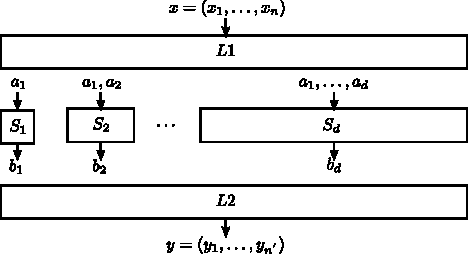
\includegraphics{image1.pdf}
\end{center}

Attacking DRegZ occurs in two phases. First, a method is developed to carefully choose $x$ so that the resulting $a = L1(x)$ affects only certain $S_i$.
Second, we derive how these $x$ are used to produce $b$ such that $y = L2(b)$ for chosen $y$.

\section{Isolating Inputs to Chosen $S_i$}

Normally with many random inputs $r_i$, $L1(r_i)$ produces vectors $a$ which span the entire $n$-dimensional space.
Let $s_i$ be the inputs where $L1(s_i) = a = (0, a_2,\ldots ,a_n)$.
The $a_1=0$ affects the dimension of $a$, $b$, and $y$ in a way that we will exploit.

With $width(a_1) = |S_1|$ bits held constant, $a$ now spans a subspace only $1/2^{|S_1|}$ the size of the entire $n$-dimensional space. $dim(a)=n-|S_1|$.
Since L1 is an invertible linear transform, there exists a counterpart subspace in $x$.

Now $b_1$ is held constant, at whatever the value $S_1$ is evaluated at $a_1=0$.
With $width(b_1) = |S_1|'$ bits held constant, b now spans a subspace only $1/2^{|S_1|'}$ the size of the entire $n'$-dimensional space. $dim(b)=n'-|S_1|'$.
Since L2 is an invertible linear transform, there exists a counterpart subspace in $y$.

But how do we find these $s_i$? For the random inputs $r_i$ already mentioned, likely their $a_i\neq 0$.
Adding $s_i$, $f(r_i+s_i)$ should differ from $f(r_i)$ in $n' - |S_i|'$ dimensions.
This is the differential attack given in [1].
To test if, for some trial vector $t$, $L1(t) = (0, a_2,\ldots , a_n)$, we do:

\begin{enumerate}
\item for each of $n'$ random inputs $r_i$, collect $f(r_i) - f(r_i + t)$ into a basis $B$.
\item return true if $dim(B) = n' - |S_1|$, false otherwise
\end{enumerate}

Now we wish to find $s_i$ such that $f(s_i) = (0, 0, a_3, \ldots , a_n)$. Since this is a subspace of $(0, a_2, \ldots , a_n)$, we may apply the above
algorithm, except the random $r_i$ are taken from the span of $(0, a_2, \ldots , a_n)$ instead of the entire $n$-space.
Iterating this way, we collect $d$ bases:

\begin{align*}
B_1 = \{x\} | L1(x) = (a_1, a_2, \ldots , a_d) \\
B_2 = \{x\} | L1(x) = (0, a_2,\ldots , a_d) \\
\ldots \\
B_d = \{x\} | L1(x) = (0,\ldots , 0, a_d) \\
\end{align*}

Now $dim(B_1)=n, dim(B_2)=n - |S_1|, \ldots ,dim(B_d)=n - \sum{|S_{i, i<d}|}$.
For any $v \in span(B_i)$, $L1(v) = (0, \ldots, 0, a_{i}, a_{i+1}, \ldots, a_n)$.

Since $B_d \subset B_{d-1} \subset B_{d-2} \subset \ldots \subset B_{1}$, the bases can be further refined by subtracting away the subset relationships.
We let $B_d$ stand independent, now $B_{d-1} = B_{d-1} - B_d$. Next $B_{d-2} = B_{d-2} - B{d-1}$, and so on until $B_1 = B_1 - B_2$.
A simple algorithm can be used to calculate the difference between two bases $B \subset A$:

\begin{enumerate}
\item $result = \{\}$
\item $temp = B$
\item $r = random(span(A))$
\item if $r \not\in span(temp)$ \\
       $result = result \cup \{r\}$
\item $temp = temp \cup \{r\}$ ($r$ possibly dependent, and not increase $dim(temp)$)
\item if($dim(A) = dim(B) \neq dim(result)$) \\
       goto step 2
\item return $result$
\end{enumerate}

Now $dim(B_1)=|S_1|, \ldots , dim(B_d)=|S_d|$.
It is tempting to think that $B_i$ needs to span vectors $v$ where $L1(v) = a$ where $a_{j, j\neq i} = 0$, which is not true for this construction.
In reality, each $B_i$ needs only to span vectors $v$ where $L1(v) = a$ that meet the following requirements:
Each $a_{j, j<i}$ must equal 0.
Each $a_{j, j=i}$ be completely controllable by choice of $v$.
And each $a_{j, j>i}$ can be random bits dependent on $a_{j, j\leq i}$.
This is because the choice $v_1 \in span(B_1)$ can be made first, dictating the value of $b_1 = S_1(a_1)$.
Yes, this sets all $a_{i, i>1}$, $S_{i, i>1}$, and $b_{i, i>1}$ randomly, but only temporarily.
Next, choose a vector $v_2 \in span(B_2)$ such that $b_2 = S_2(b_2)$ is set correctly
($S_1$ remains correct because the $a_1$ resulting from $L1(v_2)$ is 0).
Iterate this way until $S_d$ is set correctly.

\section{Adapting Inputs Towards a Plaintext $y$}
The last section left with a method to set $S_i$ to our choosing. But $b$ still remains to travel through $L2$.

Recall that evaluating $f(v), v\in span(B_i)$ produces $b$ vectors that naturally form a space.
Since $f(v), v\in B_i$ produces $a = (0, \ldots, 0, a_i, a_{i+1}, \ldots, a_d)$, all $b_{j, j<i}$ are held constant.
This means the produced vector $b$ form a subspace of the entire $n'$-space.
As an invertible linear transformation, the values $y = L2(b)$ form also a subspace.
For every $B_i'$, we want to record what subspace at $y$ can be produced.
Calculate each $B_{i}' = span(\{f(v)\})$ where $v \in span(B_{i})$. 

We now have a correspondance between vector spaces at the input ($B_i$) and vector spaces at the output ($B_i$').
Since $\sum{dim(B_{i}')} = n'$ we know that the vector spaces at output can be used together to craft any output $y$ allowable by the $S_i$.
Decomposing some $y$ into components from each vector space $B_{i}'$ can be done by collecting the vectors from 
each $B_{i}'$ into a matrix, preserving their order, and solving:

\begin{equation*}
\begin{bmatrix}
c_1, c_2, \ldots, c_{n'}
\end{bmatrix}
\begin{bmatrix}
v_1 \in B_1' \\
v_2 \in B_1' \\
\ldots \\
v_{dim(B_1')} \in B_1' \\
\ldots \\
v_{n'-dim(B_d')} \in B_d' \\
v_{n'-dim(B_d')+1} \in B_d' \\
\ldots \\
v_{n'} \in B_d' \\
\end{bmatrix}
=
\begin{bmatrix}
y
\end{bmatrix}
\end{equation*}

With c found, $y$'s component from $B_i$ is calculated as the dot product of c with the same matrix as above, except the rows pertaining
to vectors from $B_{j, j\neq i}$ are set 0:

\begin{equation*}
component_{B_i'}
=
\begin{bmatrix}
c_1 \\
c_2 \\
\ldots \\
c_{n'} \\
\end{bmatrix}
\cdot
\begin{bmatrix}
0 \\
\ldots \\
0 \\
v_{\sum_{j=1}^{i-1} dim(B_j')} \in B_i' \\
v_{\sum_{j=1}^{i-1} dim(B_j') + 1} \in B_i' \\
\ldots \\
v_{\sum_{j=1}^{i} dim(B_j') - 1} \in B_i' \\
0 \\
\ldots \\
0
\end{bmatrix}
\end{equation*}

We can now decompose any $y$ into the $d$ spaces $B_i'$.
We have also the correspondence between these $B_i'$ and the $B_i$ at input.
Thus we are equipped to adapt an input that solves for $y$ with the following algorithm:

\begin{enumerate}
\item decompose $y$ into the $d$ components from each $B_i'$
\item find $solution_1 \in span(B_1)$ such that\\
$component_1(f(solution_1))=component_1(y)$
\item find $solution_2 \in span(B_2)$ such that\\
$component_2(f(solution_1+solution_2)=component_2(y)$
\item $\ldots$
\item find $solution_d \in span(B_d)$ such that\\
$component_d(f(solution_1+,\ldots ,+solution_d)=component_d(y))$
\item return $\sum{solution_i}$
\end{enumerate}

\section*{References}
[1] Jacques Patarin, Asymmetric Cryptography with S-Boxes, pp. 1-10. \newline
[2] Giuliano Bertoletti, Algorithm for license codes (sci.crypt)

\end{document}
